\subsection{Použité programové prostředky}

\subsubsection{PostgreSQL 9.x (PostGIS)}
        \label{PostgreSQL}
        PostgreSQL je objektově-relační databázový systém s otevřeným zdrojovým
        kódem dostupný na většině platforem. Je volně k dispozici pro použití,
        modifikaci a znovu rozšíření způsobem, který si sami zvolíme. Jedná se
        o robustní, výkonný, bezpečný, kompatibilní a interoperabilní software
        s podporou a dobře komentovaným zdrojovým kódem. Vyhovuje standardům
        SQL od verze SQL 2008 a nabízí velké množství pokročilých funkcí.
        PostgreSQL je založen na architektuře klient-server, to znamená, že
        server pořád běží a čeká na dotazy klienta \citep{Momjian2001}. 

        S vývojem databázového serveru PostgreSQL začala University of
        California v Berkley již více než před 20 lety. Nyní je vyvíjen a
        udržován velkou komunitou nezávislých vývojářů. Používá licenci TPL
        (The PostgreSQL Licence), která je mírně odlišná od open-source licence
        BSD (Berkeley Distribution Software), ze které vychází
        \citep{RiggsKrossing2010}

        Řadí se mezi nejpokročilejší databáze díky schopnosti pracovat s
        velkými objemy dat, díky své rychlosti a funkcionalitě může soupeřit i
        s populárními komerčními systémy jako je Oracle, IBM DB2, Microsoft SQL
        Server 2008 a dalšími \citep{PostgreSQL2012}.

        Samotné PostgreSQL neobsahuje datové typy a funkce vhodné pro správu
        prostorových dat. K tomu je nutné přidat nástavbu PostGIS, která
        rozšiřuje databázi PostgreSQL o podporu geografických dat. PostGIS
        implementuje specifikaci „Simple Features for SQL“ konsorcia OGC.
        PostGIS umožňuje ukládání geometrických objektů (bod, linie, polygon),
        použití prostorových funkcí pro určení vzdáleností, délky linií, výměr
        a obvodu ploch, výběr indexu při spojení prostorových a atributových
        dotazů a mnoho dalších.

        PostGIS používá dva základní prostorové datové typy geography a
        geometry. Typ geography ukládá souřadnice v kartézských rovinných
        souřadnicích, kterým odpovídá souřadnicový systém WGS84. Je zejména
        vhodný pro malá území. Při výpočtu vzdálenosti dvou bodů tento datový
        typ vrátí jako výsledek nejkratší vzdálenost v kilometrech v rovině.
        Typ geometry data ukládá v polárním rovinném systému a umožňuje
        nastavit souřadnicový systém podle potřeb. Výsledkem dotazu na
        vzdálenost dvou bodů tedy bude úhel ve stupních. Po převodu do metrické
        soustavy dostaneme nejkratší vzdálenost na kouli. Při výběru datového
        typu může být rozhodující například počet funkcí, kterých typ geometry
        poskytuje mnohem více než geography, nebo velikosti daného území
        \citep{OpenGeo2012}.

        Existuje také další nástavba PostGIS Raster, která rozšiřuje ukládání a
        manipulaci s rastrovými daty, nástavba PostGIS Topology pro
        topologickou správu vektorových dat a pgRouting pro síťové analýzy.
        PostGIS je podporován velkou řadou software zabývajících se správou
        geografických dat, což také umožňuje snadnou přenositelnost a
        použitelnost jednotlivých nástaveb (příklad software podporujících
        PostGIS: QGIS, GvSIG, GRASS, ArcGIS).

        PostGIS používá mnoho běžně používaných knihoven jako GEOS (Geometry
        Engine Open Source) pro implementaci jednoduchých prostorových prvků a
        metod pro topologii, PROJ4 pro převod mezi kartografickými projekcemi
        nebo GDAL/OGR (Geospatial Data Abstraction Library) pro převod mezi
        různými vektorovými i rastrovými formáty \citep{ObeHsu2011}. PostGIS
        1.5. obsahovala přes 800 funkcí, typů a prostorových indexů
        \citep{ObeHsu2012}. Aktuální verze PostGIS\footnote{Aktuálně na
        http://postgis.refractions.net/} je 2.1.

        PostgreSQL podporuje replikaci i synchronizaci bez nutnosti další
        instalace. 

        Od verze ArcGIS 9.3. je PostgreSQL oficiálně podporovanou databází pro
        ukládání geodat v produktech ArcGIS. Při instalaci je pouze potřeba
        zajistit kompatibilitu verzí. Pro verzi ArcGIS 10.1 jsou podporované
        verze PostgreSQL 9.0 a PostGIS 1.5., pro ArcGIS 10.1
        SP1\footnote{Service Pack 1} je to PostgreSQL 9.1.3 a PostGIS 2.0
        \citep{OSGEO2013}\footnote{Zdroj a další informace na stránkách
        PostgreSQL http://trac.osgeo.org/postgis/wiki/UsersWikiPostgisarcgis
      nebo ArcGIS http://resources.arcgis.com/en/help/system-requirements/10.1/index.html\#//015100000075000000}.
    Databáze PostgreSQL se dá v ArcGIS produktech použít dvojím způsobem. Buď
    jen jako uložiště dat bez přidání geografického datového typu, nebo včetně
    datového typu, tedy včetně PostGIS knihovny. ArcSDE podporuje pouze datový
    typ PostGIS Geometry a přidává vlastní datový typ Esri St\_Geometry.
    Výhodou použivání Esri St\_Geometry je nezávislost na zvoleném databázovém
    systému, tedy snazší přenostitelnost celého řešení. 

        Práce byla testována na verzích PostgreSQL\footnote{Více na
        http://www.postgresql.org/} 9.1.4 a PostGIS 2.0.

        \subsubsection{Microsoft SQL Server Express 2008}
        \label{MSSQL}
        Microsoft SQL Server (dále MS SQL Server) je relační databázový systém vyvíjený
        společností Microsoft dostupný pro různé verze operačního systému Windows.
        Dodává se v mnoha verzích, které lze nainstalovat na různé hadrwarové platformy
        na základě odlišných licenčních modelů \citep{Whalen2008}. Podle Leitera (2009)
        SQL Server nabízí 8 základních verzí: Enterprise, Standard, Workgroup, Web,
        Express, Express Advanced Edition, Developer Edition a Compact Edition.
        Enterprise edition podporuje naprosto vše, co SQL Server nabízí, naopak verze
        Express, která je dostupná zdarma, obsahuje omezení některých funkcí a proto je
        vhodná spíše pro malé nebo začínající projekty \citep{Leiter2009}.

        Prostorová data jsou implementována jako CLR rozšíření a přidávají databázovému
        serveru dva prostorové datové typy geometry a geography. Rozdíl mezi datovými
        typy je podobný jako u PostgreSQL. První jmenovaný slouží k reprezentaci dat
        (bodů, linií, polygonů) v rovině, naproti tomu datový typ geography slouží
        ukládání stejných dat na povrchu zeměkoule. Oba typy pracují ve dvou dimenzích
        (nebere se v potaz výška). Podporuje také indexování dat, index je tvořen
        standardním B stromem \citep{Cincura2009}.

        SQL Server je podporován a používán ArcGIS produkty od začátku jeho vývoje.
        Verze ArcGIS Enterprise může být propojena s jakoukoliv uživatelem zvolenou a
        zakoupenou licencí databázového systému. Verze ArcSDE Desktop a Workgroup
        používají verzi Express, která je dostupná zdarma a podporuje většinu
        základních funkcí. Replikaci plně podporuje verze Enterprise, ostatní verze ji
        podporují pouze s omezenými funkcemi. Avšak již zmiňovaná verze Express, která
        je podporávána ArcSDE Desktop a Workgrorp, může být použita pouze slave server,
        tedy odběratelem replikovaných dat, není tedy možné do takovéto databáze
        připojené do replikačního clusteru zapisovat. Nemůže být tím, kdo poskytuje
        data k replikaci \citep{Whalen2008}. Stejně jako u PostgreSQL platí, že si
        uživatel může zvolit, zda použije datový typ, který je součastí ArcSDE, nebo
        ten, který je implementován do SQL Serveru. 

        \subsubsection{ArcSDE geodatabase}
        \label{ArcSDE}
        ArcSDE je technologie firmy Esri pro správu geoprostorových dat uložených v
        relačních databázových systémem. Jedná se o otevřenou a interoperabilní
        technologii, která podporuje čtení a zápis mnoha standardů. Využívá jako své
        nativní datové struktury standard konsorcia OGC Simple Feature a prostorový typ
        ISO pro databázové systémy Oracle, IBM DB2 a Informix. Poskytuje vysoký výkon a
        je přizpůsobena velkému počtu uživatelů \citep{Esri2006}.

        ArcSDE je prostředník pro komunikaci mezi klientem (př. ArcView) a SQL databází
        (př. PostgreSQL). Umožňuje přístup a správu dat v databázi, současnou editaci
        jedné databáze více uživateli, zajišťuje prostorový datový typ (St\_Geometry),
        dále integritu dat, dlouhé transakce a práci s verzemi \citep{Law2008}.

        Technologie ArcSDE vyžaduje dvě úrovně: databázovou a aplikační, která se
        skládá z ArcObjects a ArcSDE. Databázová úroveň zajišťuje jednoduchý, formální
        model pro uložení a správu dat ve formě tabulek, definici typů atributů
        (datových typů), zpracování dotazů či víceuživatelské transakce
        \citep{Law2008}. ArcSDE podporuje databázové systémy IBM DB2, IMB Informix,
        Oracle, Microsoft SQL, PostgreSQL \citep{Esri2013a}.

        Existují tři úrovně ArcSDE databáze: desktop (ArcSDE Desktop), skupinová
        (ArcSDE Workgroup) a podniková (ArcSDE Enterprise). Každá verze má jiné
        parametry a umožňuje různou úroveň editace \odkazObrazek{sde}. 

        \begin{figure}[H]
            \centering
            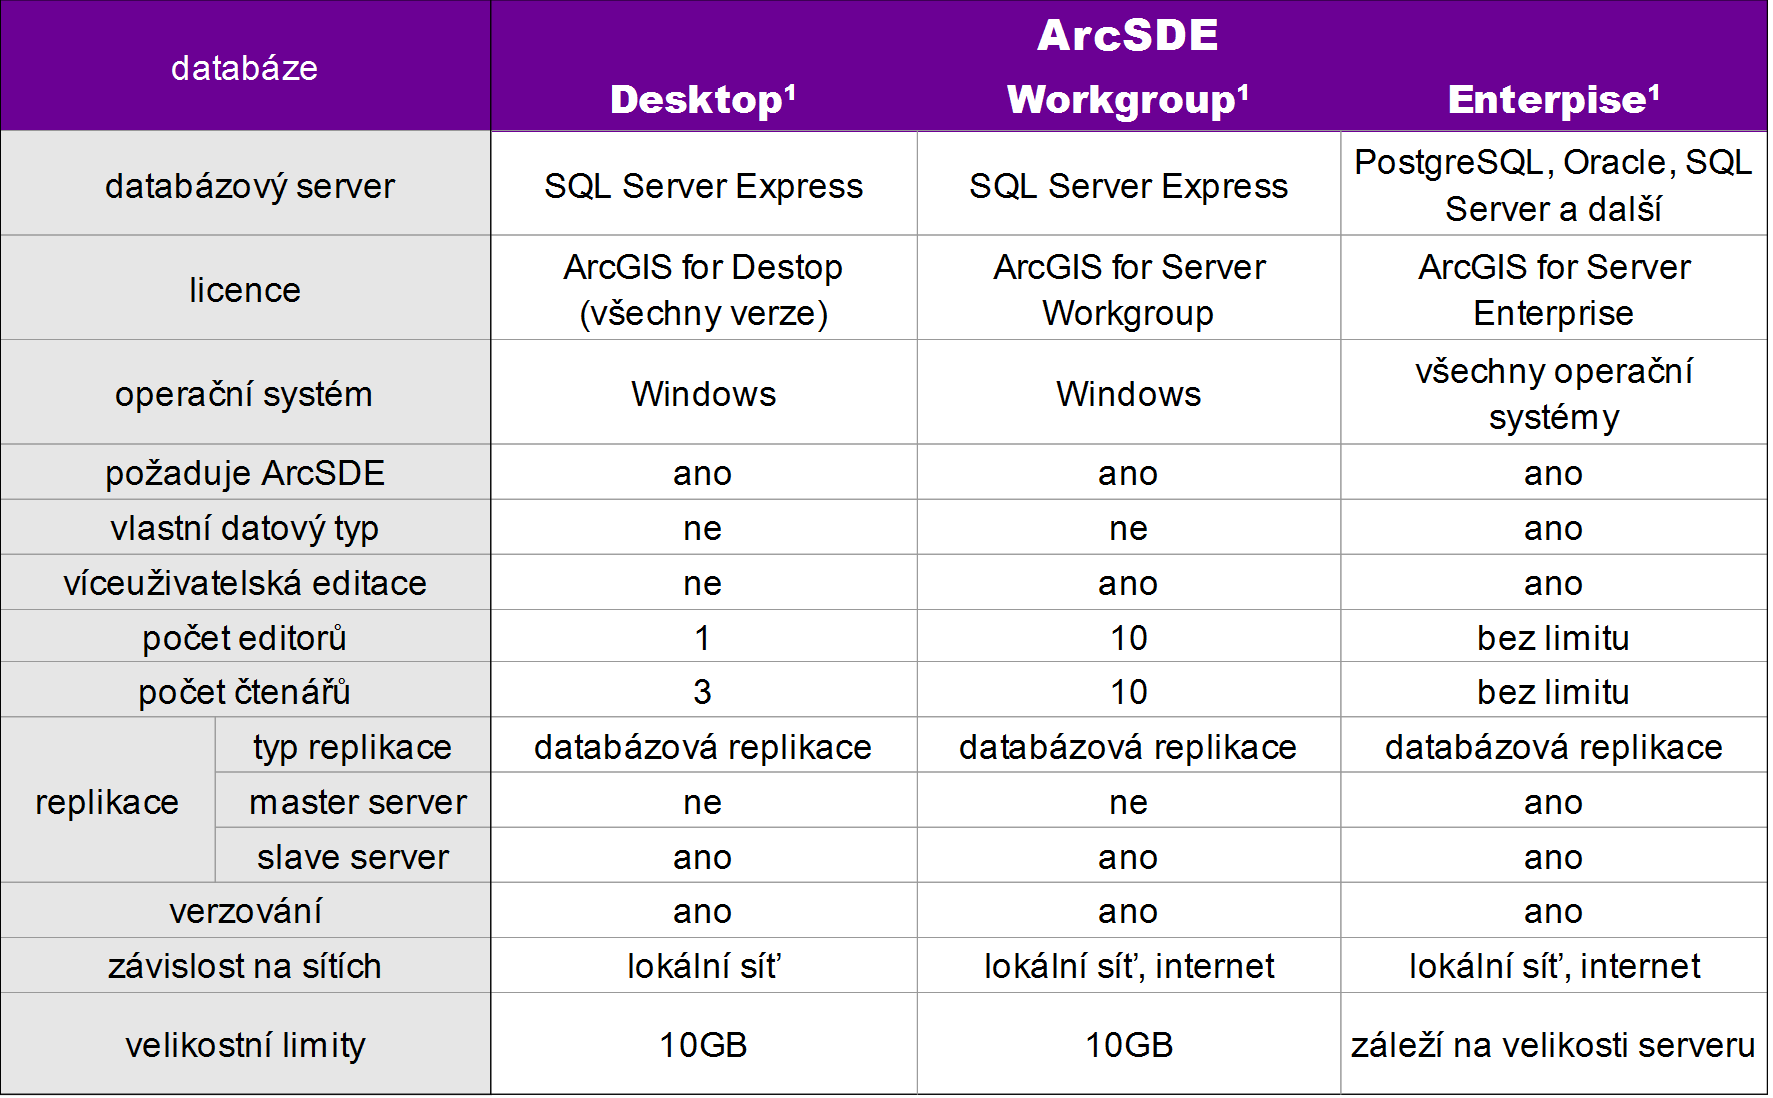
\includegraphics[width=1\textwidth]{../../../grafy/obr/tabulka_ArcSDE_primo.png}
            \caption[Přehled verzí ArcSDE, jejich parametrů a možností]{Přehled verzí ArcSDE, jejich parametrů a možností\newline \textsuperscript{1} zdroj 
        http://www.esri.com/software/arcgis/geodatabase/multi-user-geodatabase}
            \label{sde}
          \end{figure}
        
        ArcGIS 9.2 je ArcSDE Desktop spolu s databázovým systémem MS SQL Server Express
        součástí licence produktů ArcGIS for Desktop Standard a Advanced. Takovou
        databázi mohou současně používat 4 uživatelé, z toho jen jeden může databázi
        editovat, jsou však omezeni velikostí databáze.

        Součastí licence ArcGIS for Server Workgroup je ArcSDE Workgroup, která se liší
        od verze Desktop především tím, že počet uživatelů, kteří mohou součastně
        editovat nebo prohlížet databázi, je zvýšen na deset.

        Nejvyšší úroveň, ArcSDE Enterprise, je možno získat s licencí ArcGIS for Server
        Enterprise, která uživatelům přináší nejméně omezení. Mohou si vybrat z
        několika komerčních i nekomerčních databázových systémů, počet uživatelů není
        omezen, stejně jako velikost databáze.

        K ArcSDE a vybrané databázi je možno přistupovat přes ArcCatalog, není tedy
        potřeba instalace dalšího software nebo zkušenost s administrací databáze
        \citep{Esri2006}.

        Replikaci a synchronizaci dat umožňují pouze ArcSDE Enterprise a Workgroup
        \citep{Esri2013b}. Jak už bylo zmíněno v předchozí kapitole \odkazKapitola{MSSQL} Microsoft SQL
        Server Express 2008, SQL Server Express je možný použít v replikačním clusteru
        pouze jako slave server. Vzhledem k tomu, že proces replikace je implementován
        pří do ArcObjects a ArcSDE, nezáleží na konkrétním databázovém systému
        \citep{Law2008}.


